\documentclass[border=10pt]{standalone}
\usepackage{amsmath,amssymb}
\usepackage{tikz}
\usetikzlibrary{shapes.geometric, arrows.meta, positioning, calc, fit, backgrounds, decorations.pathreplacing}

\begin{document}
\begin{tikzpicture}[
    font=\sffamily,
    >=Stealth,
    node distance=1.6cm and 1.8cm,
    block/.style={draw=blue!70!black, fill=blue!8, line width=1.2pt, rounded corners=4pt, text centered, inner sep=6pt},
    reg/.style={draw=gray!80, fill=gray!20, line width=1pt, rounded corners=2pt, minimum height=1.8cm, minimum width=0.5cm, inner sep=2pt, text centered},
    ctrl/.style={draw=red!70!black, fill=red!8, line width=1.2pt, rounded corners=4pt, text centered, inner sep=6pt},
    bus/.style={line width=1.3pt, ->},
    ctrlbus/.style={line width=1pt, dashed, red!70!black, ->},
    labelstyle/.style={font=\small\sffamily, fill=white, inner sep=1.5pt}
]

    % Coordinates & Inputs
    \node (d_in) at (0, 3.2) {\textbf{d\_tile} $[0:3][0:3]$ \\ \small 16 $\times$ INT16};
    \node (u_in) at (0, 0.8) {\textbf{u\_tile} $[0:3][0:3]$ \\ \small 16 $\times$ INT16 ($U=GgG^T$)};
    \node (ctrl_in) at (0, -1.8) {\textbf{Control Inputs} \\ \small \texttt{start}, \texttt{first\_ch}, \texttt{last\_ch}, \texttt{cin\_count}};

    % Stage 1: Input Transform Unit
    \node[block, minimum width=3.4cm, minimum height=2.4cm, right=1.6cm of d_in] (in_trans) {
        \textbf{Input Transform Unit}\\
        \textbf{\texttt{input\_transform\_2d}}\\
        \vspace{0.15cm}
        \small $V = B^T d B$\\
        \footnotesize Multiplierless 1D Col $\to$ 1D Row\\
        \footnotesize Addition/Subtraction Trees
    };

    % Pipeline Reg 1 (V)
    \node[reg, right=1.2cm of in_trans] (reg_v) {\rotatebox{90}{\textbf{REG (18b)}}};

    % Delay Reg 1 (U)
    \node[reg, right=4.0cm of u_in] (reg_u1) {\rotatebox{90}{\textbf{REG (16b)}}};

    % Stage 2: Multiplier Array
    \node[block, minimum width=3.4cm, minimum height=2.8cm, right=1.4cm of reg_v, yshift=-1.2cm] (mul_array) {
        \textbf{Multiplier Array}\\
        \textbf{\texttt{multiplier\_array}}\\
        \vspace{0.15cm}
        \small $M = U \odot V$\\
        \footnotesize 16 Parallel Signed Multipliers\\
        \footnotesize INT18 $\times$ INT16 $\to$ INT34\\
        \footnotesize (Configurable 4, 8, 16 DSPs)
    };

    % Pipeline Reg 2 (M)
    \node[reg, right=1.2cm of mul_array] (reg_m) {\rotatebox{90}{\textbf{REG (34b)}}};

    % Stage 3: Channel Accumulator
    \node[block, minimum width=3.2cm, minimum height=2.4cm, right=1.2cm of reg_m] (accum) {
        \textbf{Channel Accumulator}\\
        \textbf{\texttt{channel\_accumulator}}\\
        \vspace{0.15cm}
        \small $M_{\text{accum}} = \sum_{c=1}^{C_{\text{in}}} U^{(c)} \odot V^{(c)}$\\
        \footnotesize 16 Parallel 36-bit Accumulators\\
        \footnotesize Partial Sum Storage
    };

    % Pipeline Reg 3 (Accum)
    \node[reg, right=1.2cm of accum] (reg_accum) {\rotatebox{90}{\textbf{REG (36b)}}};

    % Stage 4: Output Transform Unit
    \node[block, minimum width=3.6cm, minimum height=2.8cm, right=1.2cm of reg_accum] (out_trans) {
        \textbf{Output Transform Unit}\\
        \textbf{\texttt{output\_transform\_2d}}\\
        \vspace{0.15cm}
        \small $Y = A^T M_{\text{accum}} A$\\
        \footnotesize Multiplierless 1D Col $\to$ 1D Row\\
        \footnotesize Add/Sub Trees $\to$ \texttt{Shift(>>>6)}\\
        \footnotesize Saturation Logic to INT16
    };

    % Output
    \node[right=1.5cm of out_trans] (y_out) {
        \textbf{y\_tile} $[0:1][0:1]$\\
        \small 4 $\times$ INT16 ($2 \times 2$ Output)\\
        \small \texttt{out\_valid}
    };

    % Controller Block
    \node[ctrl, minimum width=7.5cm, minimum height=1.8cm, below=2.6cm of mul_array] (fsm_ctrl) {
        \textbf{Winograd FSM Controller (\texttt{winograd\_controller})}\\
        \small States: \texttt{IDLE} $\to$ \texttt{PROCESS} $\to$ \texttt{WAIT\_DRAIN} $\to$ \texttt{DONE}\\
        \footnotesize Handshakes: \texttt{in\_ready}, \texttt{first\_channel}, \texttt{last\_channel}, \texttt{tile\_done}
    };

    % Connecting Busses
    \draw[bus] (d_in) -- node[above, font=\footnotesize] {16 $\times$ 16b} (in_trans.west);
    \draw[bus] (in_trans.east) -- node[above, font=\footnotesize] {16 $\times$ 18b} (reg_v.west);
    \draw[bus] (reg_v.east) -- ++(0.5,0) |- node[pos=0.3, above, font=\footnotesize] {$V$ [17:0]} (mul_array.160);

    \draw[bus] (u_in) -- node[above, font=\footnotesize] {16 $\times$ 16b} (reg_u1.west);
    \draw[bus] (reg_u1.east) -- ++(0.5,0) |- node[pos=0.3, below, font=\footnotesize] {$U$ [15:0]} (mul_array.200);

    \draw[bus] (mul_array.east) -- node[above, font=\footnotesize] {16 $\times$ 34b} (reg_m.west);
    \draw[bus] (reg_m.east) -- node[above, font=\footnotesize] {$M$ [33:0]} (accum.west);
    \draw[bus] (accum.east) -- node[above, font=\footnotesize] {16 $\times$ 36b} (reg_accum.west);
    \draw[bus] (reg_accum.east) -- node[above, font=\footnotesize] {$M_{\text{accum}}$} (out_trans.west);
    \draw[bus] (out_trans.east) -- node[above, font=\footnotesize] {4 $\times$ 16b} (y_out.west);

    % Control Connections
    \draw[ctrlbus] (ctrl_in.east) -- ++(1.0,0) |- (fsm_ctrl.west);
    \draw[ctrlbus] (fsm_ctrl.north) -- node[right, font=\footnotesize] {\texttt{first\_ch\_d2, last\_ch\_d2}} (accum.south);
    \draw[ctrlbus] (fsm_ctrl.north -| reg_u1.south) -- (reg_u1.south);
    \draw[ctrlbus] ($(fsm_ctrl.north west)!0.7!(fsm_ctrl.north)$) -- ++(0,1.2) -| (in_trans.south);
    \draw[ctrlbus] ($(fsm_ctrl.north east)!0.3!(fsm_ctrl.north)$) -| (out_trans.south);

    % Top-level Boundary
    \begin{scope}[on background layer]
        \node[draw=blue!40, fill=blue!2, dashed, line width=1.5pt, rounded corners=8pt,
              fit=(in_trans) (out_trans) (y_out) (fsm_ctrl) (reg_u1) (reg_v),
              inner sep=16pt,
              label={[font=\bfseries\large\color{blue!80!black}, anchor=north west]north west:Top-Level Pipelined Winograd Accelerator Core (\texttt{winograd\_top.sv})}] (top_box) {};
    \end{scope}

\end{tikzpicture}
\end{document}
